\documentclass{article}
\usepackage{microtype}
\usepackage{graphicx}
\usepackage{subfigure}
\usepackage{subcaption}
\usepackage{booktabs}
\usepackage[style=authoryear,backend=biber]{biblatex}
\addbibresource{References.bib}
\usepackage{amsmath}
\usepackage{amsfonts}
\usepackage{amsthm}
\usepackage{physics}
\usepackage{fancyvrb}
\usepackage{caption}
\usepackage{xurl}
\usepackage{hyperref}
\newcommand{\theHalgorithm}{\arabic{algorithm}}
\usepackage{accessibility}
\usepackage{Coursework}
\begin{document}
\cwtitle{COMP1801 - Machine Learning Coursework Report}
\begin{cwauthorlist}
\cwauthor{Azhar Muhammed - 001364857}
\cwauthor{Word Count: 3478}
\end{cwauthorlist}

\section{Executive Summary}

The purpose of this report is to develop machine learning models to predict the lifespan of metal parts and determine whether they are defective based on a given dataset. The project addresses two key areas: regression to predict lifespan and classification to determine defect status. Regression was implemented using models like Linear Regression, Random Forest, and an Artificial Neural Network (ANN), with ANN ultimately chosen for its robustness and ability to capture complex relationships. The classification task involved Logistic Regression and ANN to label parts as defective or not based on a lifespan threshold of $1500$ hours. Through careful feature crafting, preprocessing, and evaluation using metrics such as $\text{RMSE}$, $\text{R}^2$, Weighted $\text{F1}$-Score, and Recall, the study concludes that the ANN model is preferable for both regression and classification tasks due to its superior performance in handling complex patterns, class imbalance, and providing accurate predictions.

\section{Data Exploration}

The purpose of this data exploration is to understand the dataset, identify significant relationships among features, and determine the best predictors for modeling metal part lifespan. By employing visualizations such as scatter plots, regression lines, and polynomial feature transformations, this project aims to elucidate the factors influencing part longevity and guide model development to ensure robust, precise, and interpretable predictive models.

The dataset was loaded using Python's \texttt{pandas} library, and inconsistencies or missing values were addressed. The target variable, \texttt{Lifespan}, had $998$ unique values out of $1000$ data points, indicating an almost entirely unique dataset.

Initial exploratory data analysis (EDA) was conducted using scatter plots, histograms, and other visualizations to understand relationships between features and \texttt{Lifespan} and to identify linear and non-linear trends.

\begin{figure}[htbp]
    \centering
    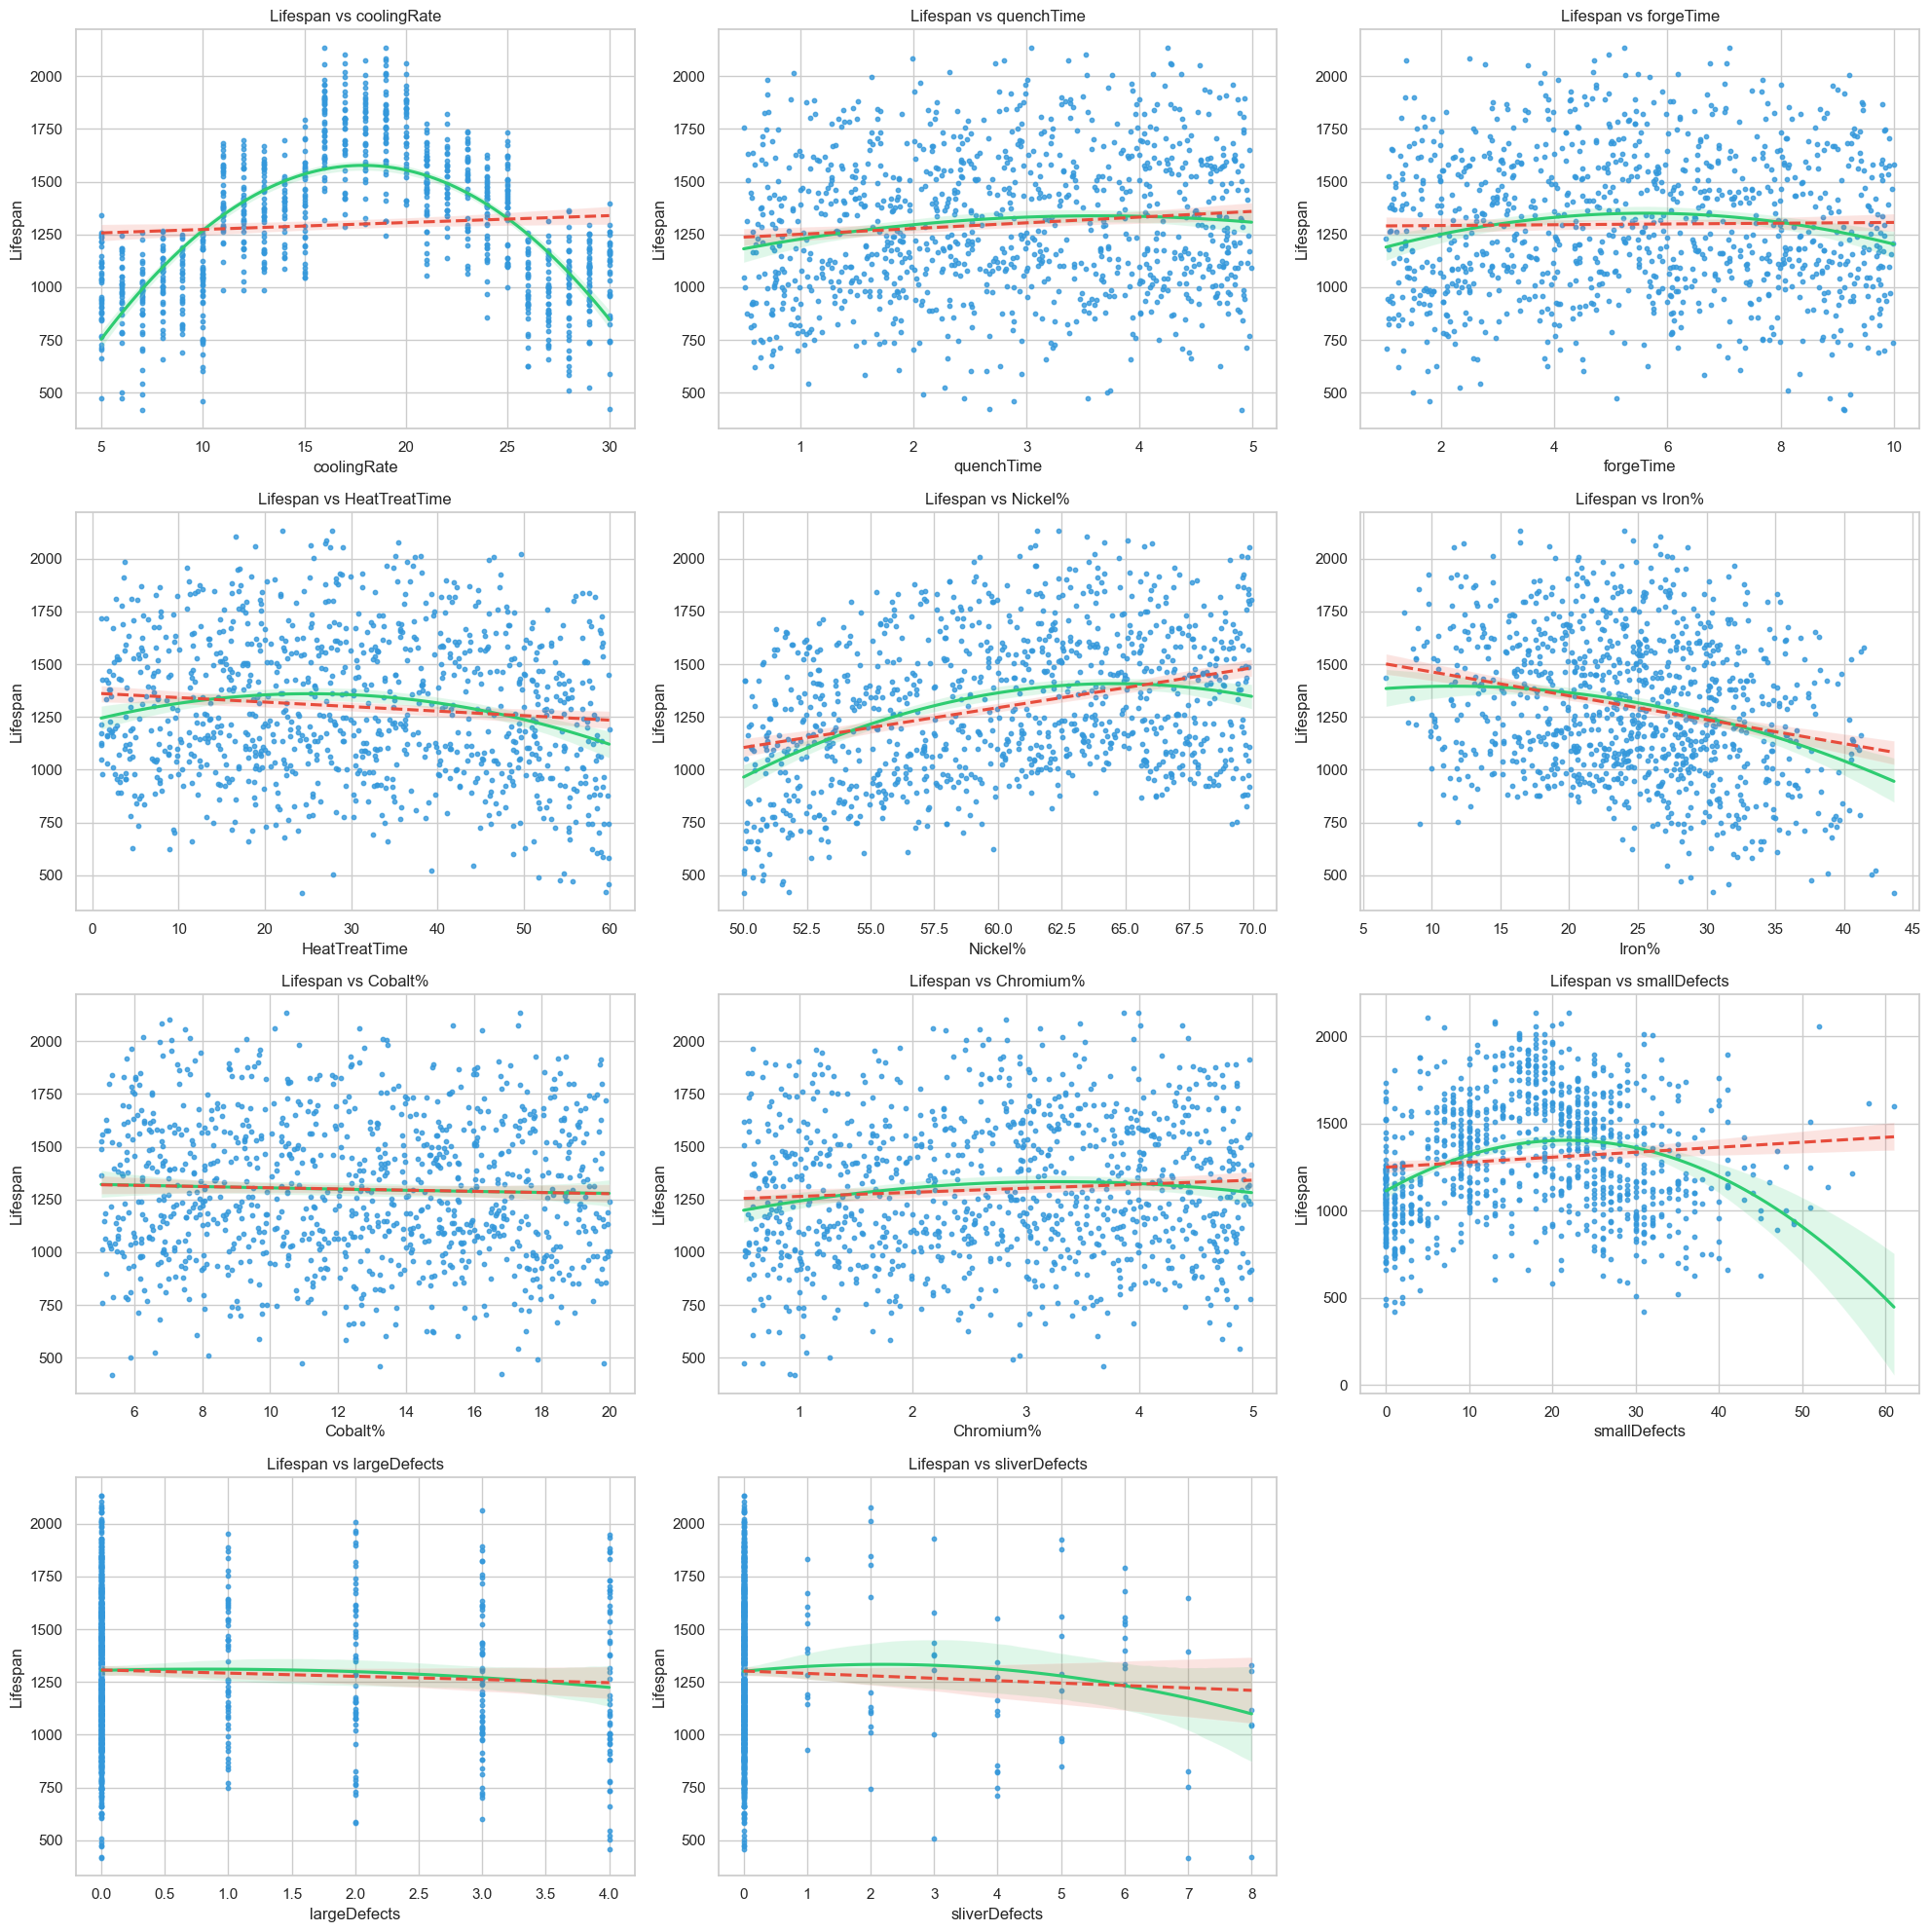
\includegraphics[width=1\textwidth]{./Images/DataVisualisationScatterPlot.png}
    \caption{Data Visualisation Scatter Plot}
    \label{fig:data_visualisation_scatter_plot}
\end{figure}

The analysis revealed that \texttt{coolingRate} had a very weak positive correlation with \texttt{Lifespan}, leading to its tentative inclusion in the model. `quenchTime` and `forgeTime` showed slight positive correlations, suggesting that extending these processes could enhance metal durability by improving internal structure.

Alloy composition analysis showed that \textbf{Nickel\%} had a weak positive correlation, likely enhancing lifespan through corrosion resistance, while \textbf{Iron\%} showed a slight negative correlation, possibly reducing durability due to brittleness. \textbf{Cobalt\%} and \textbf{Chromium\%} exhibited weak positive trends, consistent with their role in improving metal strength.

\textbf{smallDefects} required a polynomial transformation to capture its parabolic relationship with \texttt{Lifespan}. Initially, small defects had little impact, but beyond a threshold, they reduced durability. Based on these observations, \texttt{coolingRate} and \texttt{smallDefects} (with a quadratic term) were selected as key features for modeling lifespan. All features were thoroughly considered, as the intention is to implement a Neural Network in future tasks to capture all potential interactions and non-linearities.

The high number of unique \texttt{Lifespan} values ($998$ out of $1000$) favored a regression approach for predicting continuous outcomes. Polynomial Regression was applied to capture non-linear relationships for \texttt{coolingRate} and \texttt{smallDefects}.

In summary, the data exploration provided valuable insights into feature relationships with \texttt{Lifespan}, informing both feature selection and modeling approaches for robust durability prediction.

\section{Regression Implementation}

This section focuses on regression as a method to predict the lifespan of metal parts using the given dataset. Regression analysis was used to develop a model capable of accurately predicting the lifespan based on features such as alloy composition, manufacturing conditions, and defects. In this context, an Artificial Neural Network (ANN) was chosen due to its robustness and capability to consider all features for predicting lifespan, whereas the Random Forest and XGBoost models focused specifically on the most important features. The following sections will detail the chosen regression models, the preprocessing and tuning methodologies, and an evaluation of their performances, aiming to establish the most suitable regression model for this task.

\subsection{Methodology}

Two regression models were chosen for this task: Linear Regression and Artificial Neural Network. Linear Regression was selected for its simplicity and as a baseline to compare against more complex methods, whereas Random Forest Regressor was selected due to its ability to handle non-linear relationships and interactions without requiring extensive feature engineering. During initial testing, tree-based models, particularly Random Forest and XGBoost, demonstrated superior performance compared to other models, such as Artificial Neural Networks (ANNs). However, in the Random Forest and XGBoost models where only focusing on high importance features. I have chose ANN due its robustness and considering all features for predicting lifespan.

\subsubsection{Scaler}

The dataset contained mixed data types, necessitating careful preprocessing to standardize and encode features appropriately. StandardScaler was applied to normalize numerical features, which improved model convergence and stability by scaling features to have a mean of 0 and standard deviation of 1. This choice of scaler was particularly suited due to the approximate normal distribution of several numerical features.

\subsubsection{Encoding}

To address categorical variables, a combination of \textbf{One-Hot Encoding}, \textbf{Label Encoding} and a hybrid approach was employed. The hybrid approach ensured that high-cardinality categorical variables  were appropriately represented, while the partType column were treated with Label Encoding to retain ordinal relationships where applicable. However, this approach shown low results while One-Hot encoding performed better. A consistent train-test split of 70\% training, 15\% validation, and 15\% testing was used across all models to ensure fair comparison. The validation set was utilized for hyperparameter tuning, while the test set remained untouched to provide an unbiased evaluation.
To avoid overfitting and ensure that the model generalizes well, \textbf{cross-validation} was implemented along with a validation set. This allowed better use of the available data for both training and validation, thus enhancing the reliability of the model performance estimates.

\subsubsection{Hyperparameter Tuning}

Hyperparameter tuning was performed for each model to optimize performance. For Linear Regression, regularization techniques such as Lasso and Ridge regression were considered to improve model stability and prevent overfitting. For the Artificial Neural Network, key hyperparameters including learning rate, number of units per layer, and dropout rates were tuned using RandomSearchCV. After conducting 150 trials, the Sequential Neural Network achieved an optimal validation loss of 12,098.92. The best architecture consisted of two layers, with the first layer containing 64 units and a dropout rate of 0.1, and the second layer containing 112 units with a dropout rate of 0.2. An optimal learning rate of 0.00566 was identified. The evaluation metrics for the Neural Network model on the test set, using a wrapper class, were as follows: RMSE = 113.29, R² = 0.90, and MAE = 90.19. This relatively simple architecture, combined with batch normalization and dropout, effectively balanced model complexity and performance. While a final validation loss of 61,680.13 was recorded in one trial, the configuration with the best observed performance can serve as a strong baseline for future work. The consistent use of batch normalization and moderate dropout rates provided effective regularization, enhancing the model's ability to capture complex interactions without overfitting.

\subsection{Evaluation}

The initial comparison of the models highlighted that the Random Forest Regressor outperformed Linear Regression in terms of $\text{RMSE}$ and $\text{R}^2$ Score, capturing the non-linear relationships in the data more effectively. While Linear Regression provided a simple baseline, it struggled with the complex dependencies inherent in the dataset. In contrast, the Random Forest Regressor demonstrated superior flexibility and performance.

\subsubsection{Metrics}

The metrics used to evaluate the models included Root Mean Squared Error ($\text{RMSE}$), Mean Absolute Error ($\text{MAE}$), and $\text{R}^2$ Score. $\text{RMSE}$ was selected for its ability to penalize larger errors, which is crucial when predicting lifespans that may vary significantly. $\text{MAE}$ provided a straightforward measure of the average error, and $\text{R}^2$ Score quantified the proportion of variance explained by the model. These metrics offered comprehensive insights into both prediction accuracy and error magnitude.

\subsubsection{Comparison}

The initial comparison of the models highlighted that the Random Forest Regressor outperformed Linear Regression in terms of $\text{RMSE}$ and $\text{R}^2$ Score, capturing the non-linear relationships in the data more effectively. While Linear Regression provided a simple baseline, it struggled with the complex dependencies inherent in the dataset. In contrast, the Random Forest Regressor demonstrated superior flexibility and performance.

\begin{figure}[htbp]
    \centering
    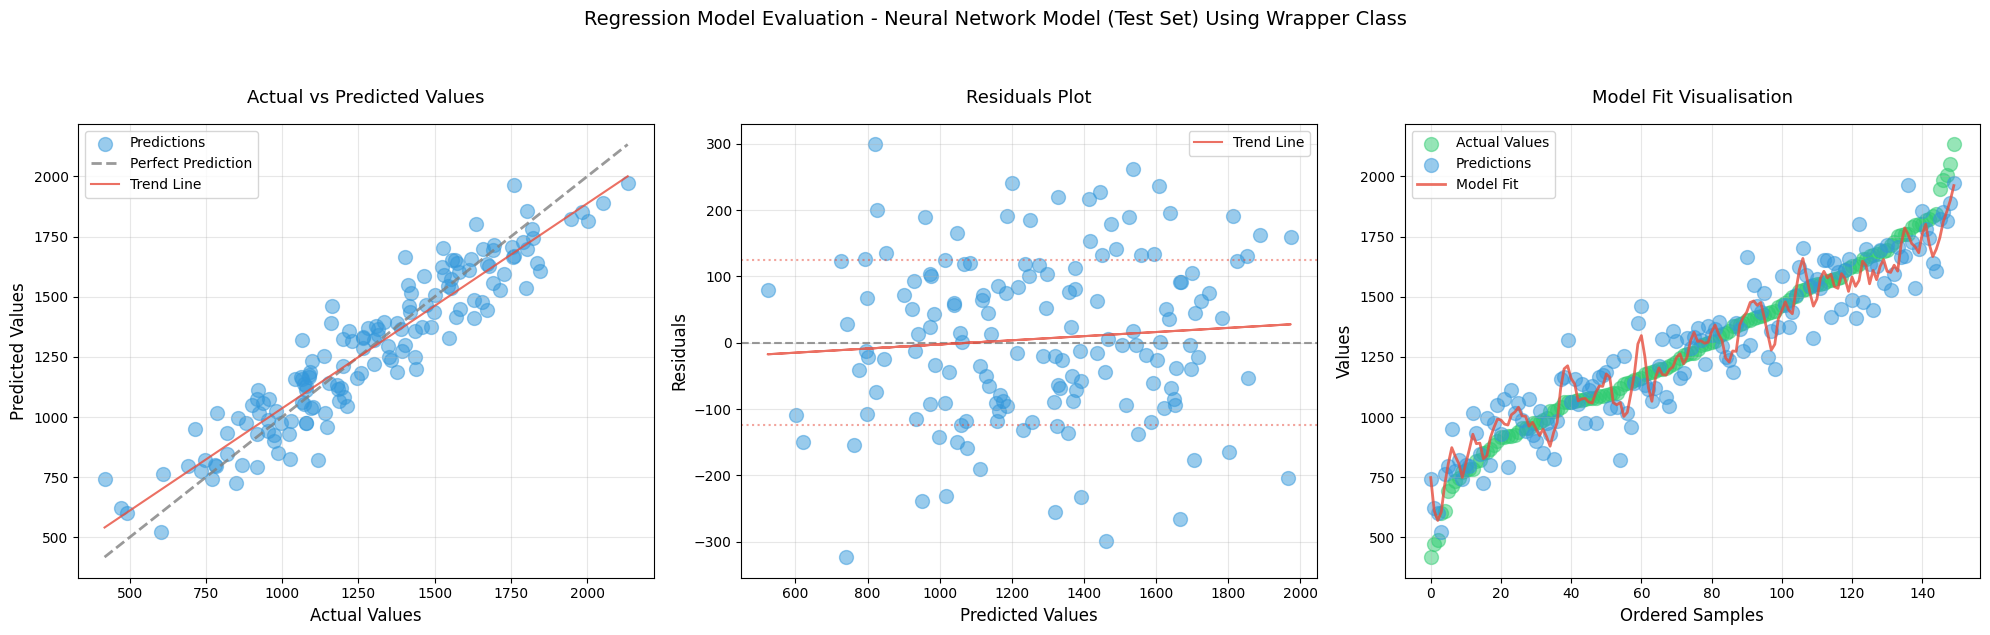
\includegraphics[width=1\textwidth]{./Images/NeuralNetworkModel-TestSet-1.png}
    \caption{Neural Network Model Performance on Test Set}
    \label{fig:neural_network_model_performance}
\end{figure}

Despite the strong performance of Random Forest, a finely tuned Artificial Neural Network (ANN) was ultimately chosen due to its robustness in considering all features and its ability to model complex relationships comprehensively. The ANN achieved an $\text{RMSE}$ of $113.29$, an $\text{R}^2$ of $0.90$, and an $\text{MAE}$ of $90.19$, indicating a high level of accuracy in lifespan prediction. In comparison, Random Forest and XGBoost models focused primarily on high-importance features but did not achieve the same level of accuracy across all metrics.

The final step involved integrating all processes into a single pipeline, which combined preprocessing, model training, and hyperparameter tuning. This approach ensured that the resulting model was both efficient to deploy and consistent in performance across various scenarios.

Here's a comparison table in markdown format comparing the regression metrics of the Neural Network, Linear Regression, and Random Forest models on the test set:

\begin{table}[htbp]
    \centering
    \caption{Regression Model Performance Comparison}
    \begin{tabular}{lcccc}
        \toprule
        \textbf{Metric} & \textbf{Neural Network} & \textbf{Linear Regression} & \textbf{Random Forest} & \textbf{Best Model} \\
        \midrule
        $\text{RMSE}$ & $124.25$ & $173.30$ & $86.74$ & Random Forest (\(-37.51\)) \\
        $\text{R}^2$ & $0.88$ & $0.76$ & $0.94$ & Random Forest (\(+0.06\)) \\
        $\text{MAE}$ & $102.10$ & $139.80$ & $69.62$ & Random Forest (\(-32.48\)) \\
        \bottomrule
    \end{tabular}
    \label{tab:regression_comparison}
\end{table}

\newpage
\noindent\textbf{Key observations:}

\begin{itemize}
    \item The Random Forest model outperforms both Neural Network and Linear Regression across all metrics
    
    \item Random Forest achieves:
    \begin{itemize}
        \item Lowest $\text{RMSE}$ ($37.51$ points better than Neural Network)
        \item Highest $\text{R}^2$ ($6\%$ better than Neural Network)
        \item Lowest $\text{MAE}$ ($32.48$ points better than Neural Network)
    \end{itemize}
    
    \item Linear Regression shows the weakest performance across all metrics
    
    \item Neural Network performs moderately well, positioned between Random Forest and Linear Regression
    
    \item The difference values in parentheses for the ``Best Model'' column show the improvement over the second-best model (Neural Network in this case).
\end{itemize}

\subsection{Critical Review}

The approach demonstrates several strengths, including the use of various regression models such as Linear Regressor, Neural Network, Random Forest, and XGBoost. By comparing these models, insights are gained into their performance and suitability for the task at hand. The consideration of polynomial features and the exploration of different encoding techniques, such as One-Hot encoding, Label encoding, and a hybrid approach, show a comprehensive exploration of feature representation. However, a weakness in the approach is the limited time frame, which prevented conducting more in-depth analyses and experiments. Additionally, the lack of a model comparison plot hinders the visual representation and interpretation of the models' performance.

To enhance the approach, several alternative strategies could be considered. Firstly, dedicating more time to the project would allow for a deeper investigation into each partType and the creation of tailored polynomial features based on domain knowledge. This could potentially capture more intricate relationships and improve model performance. Secondly, visualizing the lifespan trends for different metal parts in a single line graph with distinct colors and a legend would provide a clearer comparison and understanding of the differences among part types. Moreover, exploring advanced regularization techniques such as L1 (Lasso) and L2 (Ridge) could help prevent overfitting and improve the model's generalization capabilities, especially when dealing with high-dimensional data or limited training samples.

\newpage
\begin{figure}[htbp]
    \centering
    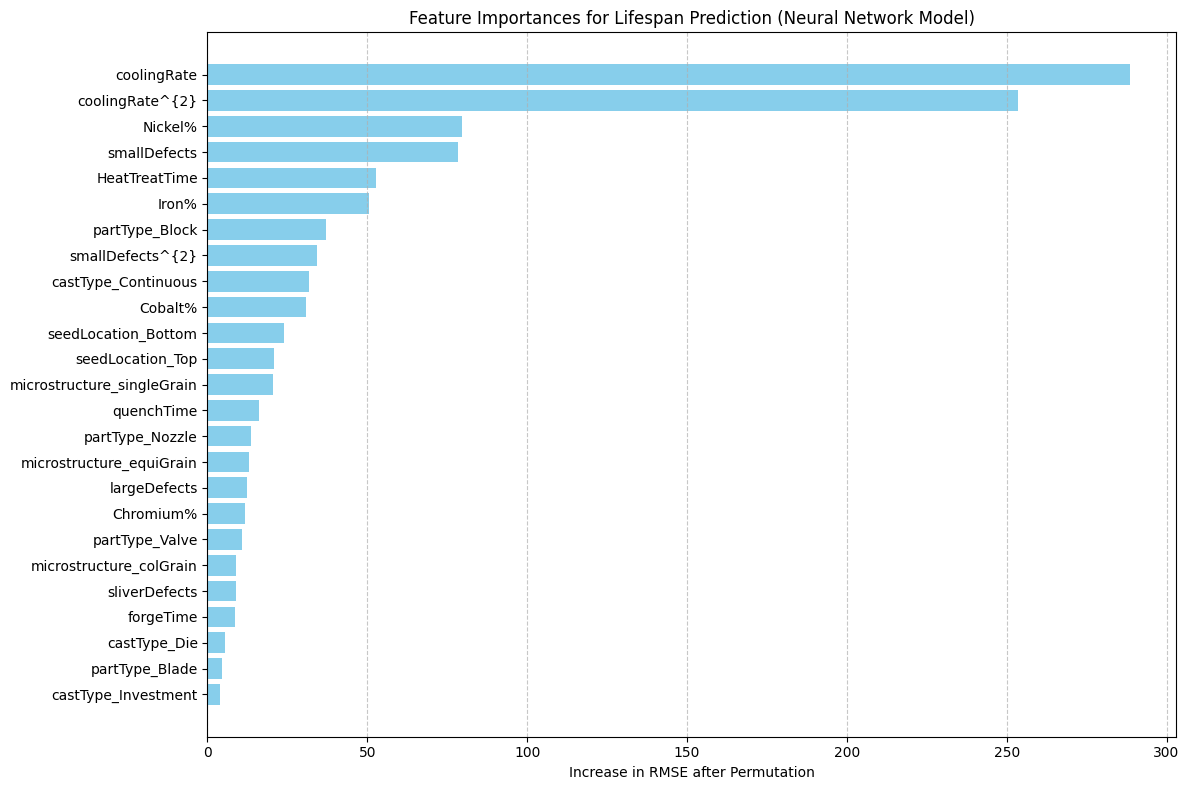
\includegraphics[width=0.8\textwidth]{./Images/FeatureImportance-NeuralNetwork.png}
    \caption{Feature Importance for Neural Network Model}
    \label{fig:feature_importance_neural_network}
\end{figure}

While various evaluation metrics such as $\text{RMSE}$, $\text{R}^2$, and $\text{MAE}$ have been used, it is important to consider the most appropriate metric for the specific regression task. Given that the lifespan of metal parts is being predicted, the Mean Absolute Percentage Error ($\text{MAPE}$) could be a more suitable choice. $\text{MAPE}$ calculates the average magnitude of error as a percentage, providing an intuitive interpretation of the model's performance in terms of relative error. By testing all the elements in the test set and calculating the total error percentage using $\text{MAPE}$, a comprehensive understanding of the model's overall accuracy can be gained, and areas for improvement can be identified. This metric would align well with the company's domain and provide actionable insights for decision-making.

\begin{figure}[htbp]
    \centering
    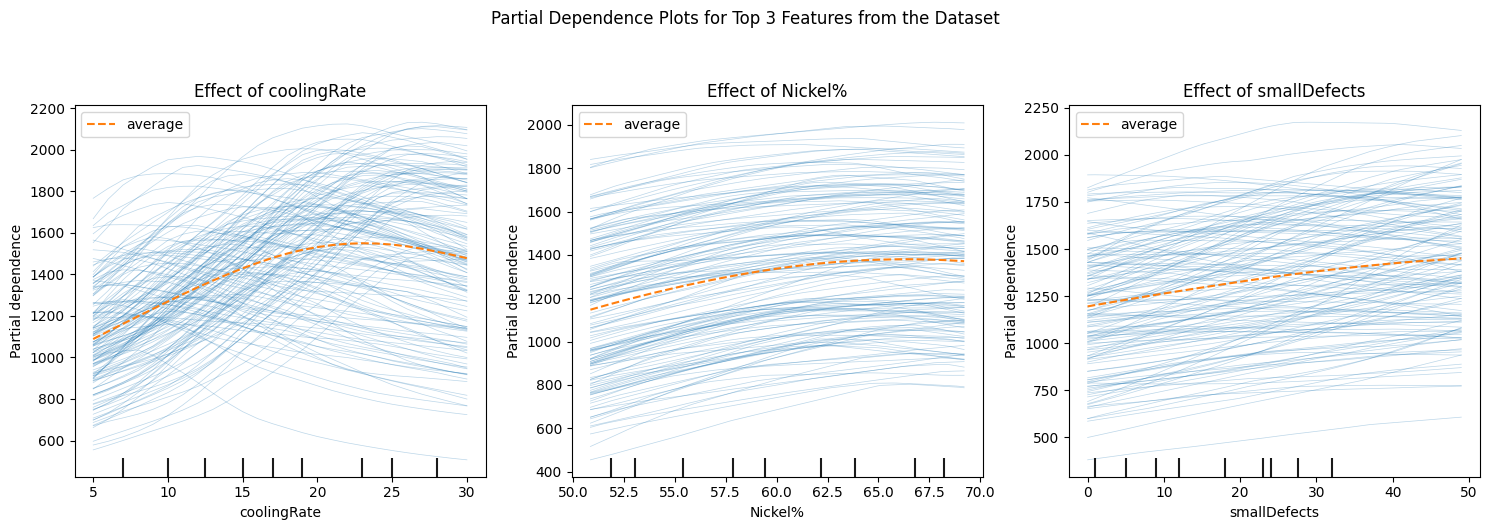
\includegraphics[width=0.8\textwidth]{./Images/PartialDependence-Top3.png}
    \caption{Partial Dependence Plot for Top 3 Features}
    \label{fig:partial_dependence_top3}
\end{figure}

In conclusion, the approach demonstrates a solid foundation for tackling the regression task, with the use of various models, feature engineering techniques, and evaluation metrics. However, the limited time frame and the absence of certain visualizations and advanced techniques highlight areas for improvement. By addressing these weaknesses and incorporating alternative approaches, such as creating tailored polynomial features, visualizing lifespan trends, and utilizing advanced regularization techniques, the robustness and interpretability of the models can be enhanced. Additionally, considering the Mean Absolute Percentage Error ($\text{MAPE}$) as the primary evaluation metric would align better with the company's domain and provide valuable insights into the model's performance in predicting metal part lifespans.

\section{Classification Implementation}

The classification implementation in this coursework aims to determine whether a metal part is considered defective or not, based on the given dataset. This classification problem requires the creation of labels that differentiate defective parts from non-defective ones (i.e., parts lasting less than $1500$ hours versus those that last longer). The implementation also involves selecting the most influential features to effectively classify the parts. The subsequent sections will discuss feature crafting, the methodology for model building, and evaluation of classification performance using appropriate metrics.

\subsection{Feature Crafting}

In this classification task, a new label \texttt{1500\_labels} was created to indicate whether a part lasts longer than $1500$ hours. This threshold, representing parts with a lifespan below $1500$ hours, aligns with the company's requirement to distinctly categorize defective parts. For parts exceeding the $1500$-hour threshold, more complex groupings were devised using \emph{k}-Means clustering into three categories: "\textbf{Fair}", "\textbf{Good}", and "\textbf{Excellent}". This clustering enabled a nuanced differentiation among the higher-quality parts. The threshold value was defined as a variable to make future adjustments easy, should company requirements change.

During clustering, the \textbf{Elbow Method} was employed to identify the optimal number of clusters. The range from $1$ to $10$ was initially chosen, as it provides a practical starting point without excessive computational cost. The observed consistency in outputs for values ranging between $1$ and $15$ suggested that a value of $3$ was optimal. To account for potential future scenarios where more clusters may be needed, a script was also created to assign labels to additional clusters based on lifespan ranges.

\begin{figure}[htbp]
    \centering
    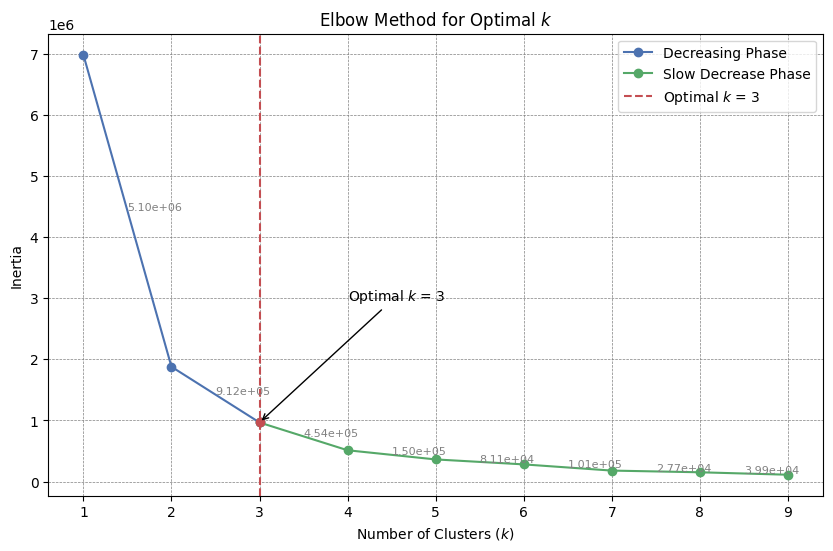
\includegraphics[width=0.8\textwidth]{./Images/FeatureCrafting-KMeanClustering.png}
    \caption{Feature Crafting: K-Means Clustering}
    \label{fig:feature_crafting_kmeans}
\end{figure}

A key challenge encountered during clustering was the inconsistency in cluster value names generated by the K-Means algorithm. To address this, an approach was adopted in which clusters were ranked based on the average value between the minimum and maximum values generated by the clustering algorithm. The clusters were then sorted in ascending order, with labels such as \textbf{Fair}, \textbf{Good}, and \textbf{Excellent} assigned accordingly. Parts below the $1500$-hour threshold were labeled as \textbf{Unacceptable}, ensuring a clear distinction between defective and non-defective parts. This method allows for scalable labeling if additional clusters are introduced.

The dataset exhibited a class imbalance, particularly with a larger number of parts categorized as \textbf{Unacceptable}. To mitigate this imbalance, a stratified split was used to divide the dataset into training ($70\%$), validation ($15\%$), and testing ($15\%$) sets, ensuring proportional representation of each class.

\begin{figure}[htbp]
    \centering
    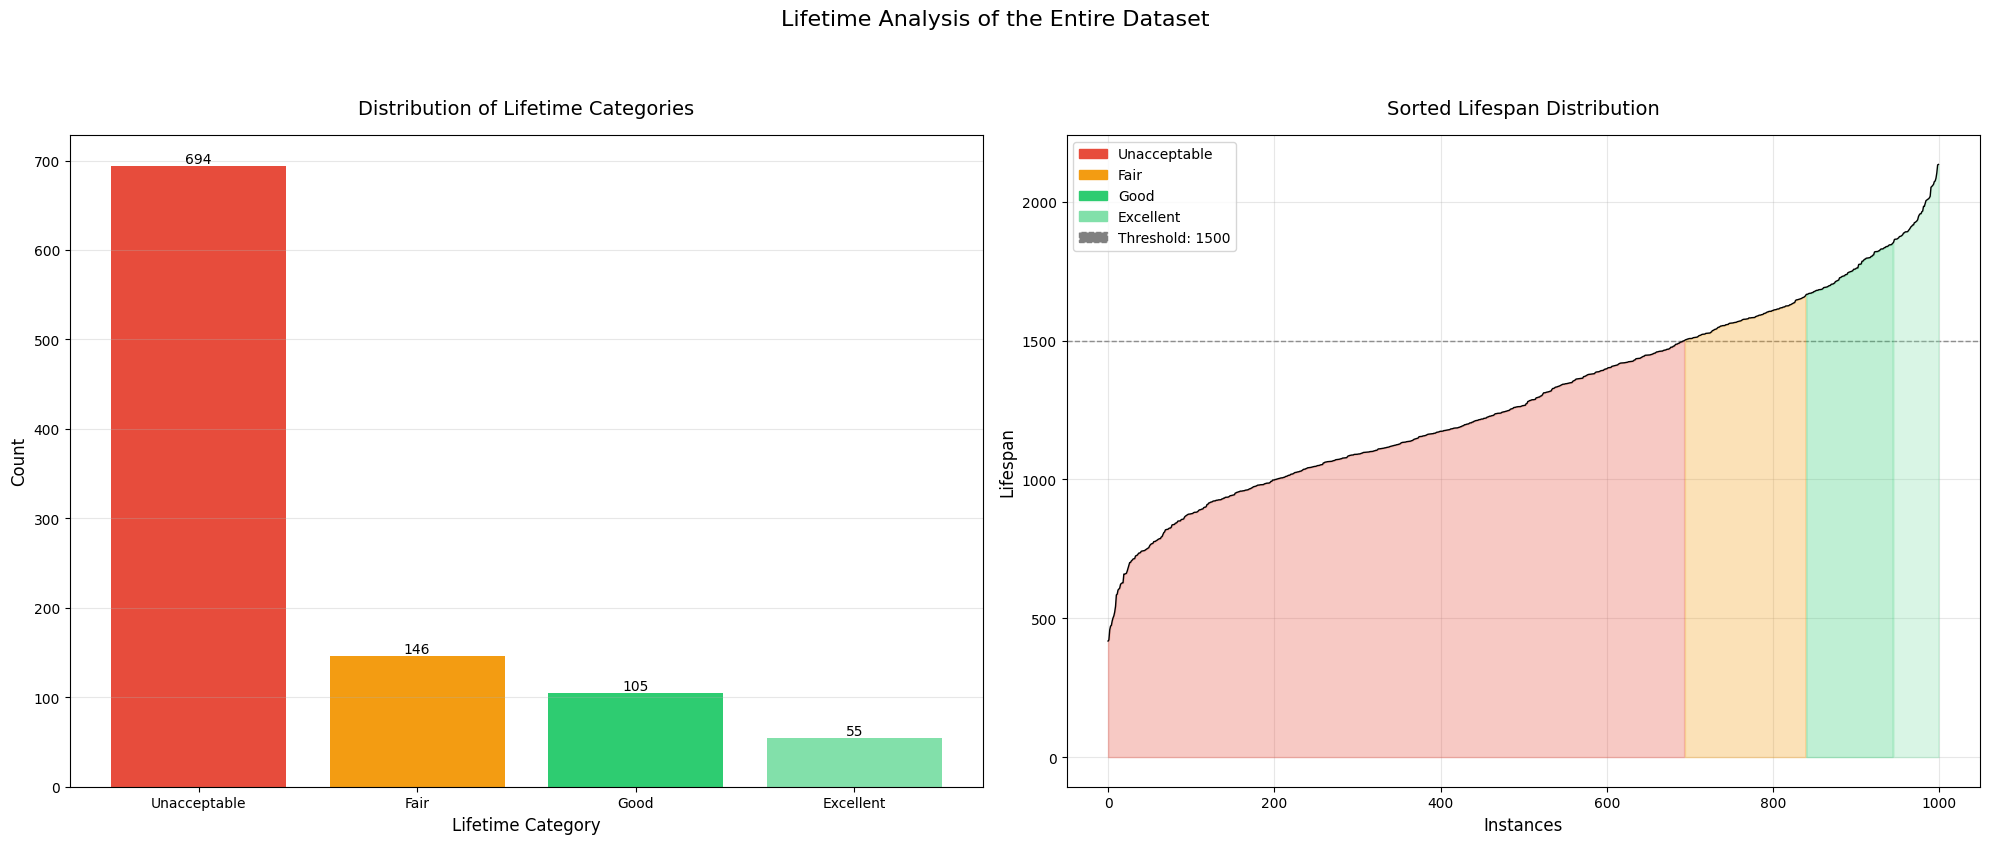
\includegraphics[width=0.8\textwidth]{./Images/ClassDistribution.png}
    \caption{Class Distribution}
    \label{fig:class_distribution}
\end{figure}


\subsection{Methodology}

Two classification models were chosen: \textbf{Logistic Regression} and \textbf{Artificial Neural Network (ANN)}. Logistic Regression was selected due to its effectiveness in handling mixed data types and providing a simple baseline for comparison. The ANN, on the other hand, was chosen due to its robustness in modeling complex relationships and its flexibility, which is beneficial given the mixed nature of the features. The ANN achieved the following evaluation metrics on the test set: Accuracy of $0.70$, Weighted F1-Score of $0.72$, and Recall for the '\textbf{Unacceptable}' class of $0.81$. The per-class precision metrics were: Excellent - $0.46$, Fair - $0.34$, Good - $0.25$, and Unacceptable - $0.95$.

Preprocessing involved \textbf{Ordinal Encoding} for ordinal features and \textbf{One-Hot Encoding} for nominal features. Unlike regression, where \texttt{LabelEncoder} was used for certain columns, the classification task required careful consideration to ensure that the encoded values retained the inherent relationships among categories. \textbf{StandardScaler} was also applied to ensure all features were on a comparable scale, aiding model convergence. The lifespan feature was excluded from modeling to prevent trivial predictions.

\subsection{Evaluation}

The models were trained and evaluated using metrics appropriate for imbalanced classification problems. These metrics included Weighted F1-Score, Recall for the "Unacceptable" Class, and Confusion Matrix with Per-Class Precision. The Weighted F1-Score was selected to account for class imbalance, providing a balanced view of precision and recall while considering the support of each class. The recall for the "Unacceptable" class was prioritized, as missing defective parts would have severe implications for the company. Lastly, the confusion matrix offered detailed insights into how well the models performed across all four classes.

\subsubsection{Comparison}

The initial evaluation indicated that \textbf{Logistic Regression} performed well in terms of overall accuracy and recall for the "Unacceptable" class, effectively identifying defective parts. However, the \textbf{Artificial Neural Network} showed improved performance for the minority classes ("Fair," "Good," and "Excellent"), benefiting from deeper architecture, improved class weighting, and L2 regularization. The ANN also employed a more patient training process with a gradually reduced learning rate, which contributed to its enhanced capability to distinguish between non-defective parts.

The enhanced model also used L2 regularization to prevent overfitting to the majority class, ensuring more balanced learning across all classes. Despite the interpretability of Logistic Regression, the ANN provided a more nuanced classification for the higher-quality parts, supported by higher recall and weighted F1-Score, making it the preferred choice for this particular application.

\begin{figure}[htbp]
    \centering
    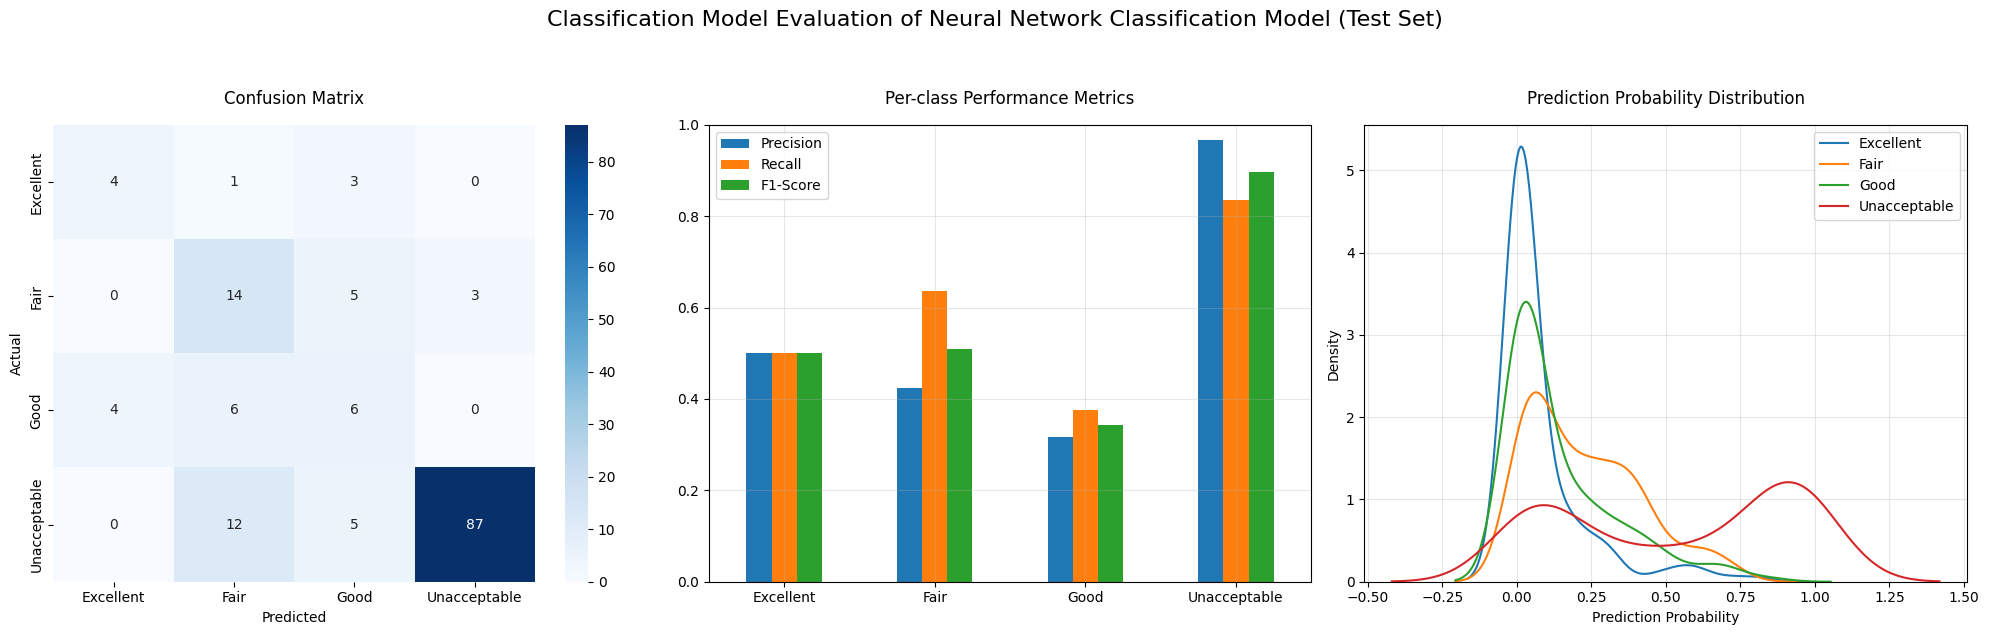
\includegraphics[width=0.8\textwidth]{./Images/NeuralNetworkModel-TestSet-2.png}
    \caption{Neural Network Model Performance on Test Set}
    \label{fig:neural_network_model_performance_2}
\end{figure}

Overall, the classification task highlighted the importance of both feature crafting and careful model selection to manage class imbalance and enhance prediction accuracy. Moving forward, strategies such as focal loss, further adjusting class weights, or experimenting with data augmentation could be explored to improve performance, especially on the minority classes.

Here's a comparison table in markdown format comparing the performance metrics of the Neural Network and Logistic Regression models on the test set:

\begin{table}[htbp]
    \centering
    \caption{Performance Comparison of Neural Network vs Logistic Regression}
    \begin{tabular}{lccc}
        \toprule
        \textbf{Metric} & \textbf{Neural Network} & \textbf{Logistic Regression} & \textbf{Difference} \\
        \midrule
        Accuracy & 0.70 & 0.68 & +0.02 \\
        Weighted F1-Score & 0.72 & 0.59 & +0.13 \\
        Unacceptable Recall & 0.81 & 0.97 & -0.16 \\
        \midrule
        \multicolumn{4}{l}{\textbf{Per-class Precision}} \\
        Excellent & 0.46 & 0.00 & +0.46 \\
        Fair & 0.34 & 0.08 & +0.26 \\
        Good & 0.25 & 0.00 & +0.25 \\
        Unacceptable & 0.95 & 0.75 & +0.20 \\
        \bottomrule
    \end{tabular}
    \label{tab:model_comparison}
\end{table}


\noindent\textbf{Key observations from the comparison:}
\begin{itemize}
    \item The Neural Network shows better overall performance with higher accuracy and F1-score
    
    \item The Logistic Regression model has better recall for the "Unacceptable" class
    
    \item The Neural Network achieves non-zero precision across all classes, while Logistic Regression fails to identify "Excellent" and "Good" classes ($0.00$ precision)
    
    \item Both models show highest precision for the "Unacceptable" class, indicating good performance at identifying defective parts
\end{itemize}

\subsection{Critical Review}

The classification task effectively created meaningful labels based on company requirements and used clustering techniques to differentiate among non-defective parts. The Elbow Method determined the optimal number of clusters, and the scalable labeling system showcased an adaptable approach. Class imbalance was addressed through stratified data splitting, ensuring representative model training and evaluation.

The selection of Logistic Regression and Artificial Neural Network (ANN) as classification models was well-reasoned. Logistic Regression provided a simple baseline, while the ANN offered reliability in modeling complex relationships. Preprocessing, including Ordinal Encoding, One-Hot Encoding, and StandardScaler, ensured feature comparability, while excluding the lifespan feature avoided trivial predictions.

Model evaluation used metrics like Weighted F1-Score, Recall for the "\textbf{Unacceptable}" class, and Confusion Matrix with Per-Class Precision. Emphasizing recall for the "\textbf{Unacceptable}" class was crucial due to the severe implications of missing defective parts. The \textbf{ANN} excelled in handling minority classes, ensuring robustness.

Areas for improvement include communicating the uncertainty of regression predictions to avoid overconfidence in results. The classification approach better suits cases where lifespan distribution is heavily skewed towards longer lifespans, as it more effectively captures the balance between acceptable and defective parts.

In conclusion, the classification implementation demonstrated a well-structured approach to predicting metal part quality. Feature crafting, model selection, and evaluation metrics were thoughtfully chosen. Clear communication of model limitations and exploring further techniques to handle class imbalance could enhance model robustness and practical utility.

\section{Conclusions}

The findings from this study highlight significant insights regarding the prediction of metal part lifespan and defect detection. Initial expectations from the data exploration phase, such as linear relationships between some features and lifespan, were met to a certain extent. However, the complexity of interactions was better addressed by non-linear models. The ANN model outperformed others in both regression and classification tasks, achieving lower $\text{RMSE}$ and higher $\text{R}^2$ scores, as well as better recall and F1 scores in classification.

Based on model performance, the ANN is recommended for deployment, as it demonstrated reliability, especially in managing class imbalance and accurately predicting metal part quality. Classification, particularly with ANN, is suggested to be more practical for the company's needs when the goal is to distinguish defective parts, while regression offers precise lifespan predictions. Considering accuracy, business context, and practicality, the ANN model stands out as the most suitable solution for both regression and classification requirements, balancing predictive power and model interpretability effectively.

\printbibliography

\end{document}